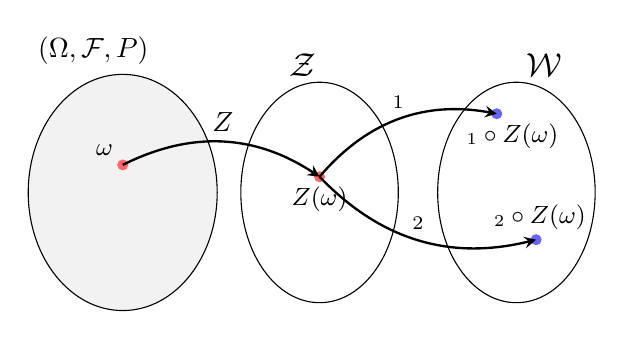
\begin{tikzpicture}[>=stealth, scale=0.5]
    % Nodes for sample space
     \def\xRadius{2.4}
     \def\yRadius{3}
     % The underlying probability space
     \draw[fill=gray!10] (-4, 0) ellipse (\xRadius cm and \yRadius cm);
     % Label
     \node[anchor=south west] at (-4-\xRadius, \yRadius) {$(\Omega, \mathcal{F}, \mathbb{P})$};
     % Observation Space $\mc{Z}$
     \draw (1, 0) ellipse (2 cm and 2.8 cm);
     % Label
     \node[anchor=south west] at (0,2.7) {\large $\mathcal{Z}$};
     % Copy of the Observation Space $\mc{Z}$
     \draw (6, 0) ellipse (2 cm and 2.8 cm);
     % Label
     \node[anchor=south west] at (6,2.7) {\large $\mathcal{W}$};

   \fill[color=red!60] (-4, 0.7) circle (4pt); % Point inside the first ellipse
   \node[above left] at (-4, 0.7) {\small$\omega$};

   \fill[color=red!60] (1, 0.4) circle (4pt); % Point inside the second ellipse
   \node[below] at (1, 0.4) {\small$Z(\omega)$};
   \fill[color=blue!60] (5.5, 2.0) circle (4pt); % Point inside the third ellipse
   \fill[color=blue!60] (6.5, -1.2) circle (4pt); % Point inside the third ellipse
   \node[below] at (5.9, 2.0) {\small $\Tau_1 \circ Z(\omega)$};
   \node[above] at (6.6, -1.2) {\small $\Tau_2 \circ Z(\omega)$};
   
   % Curved Line - Mapping Z
   \draw[->, bend left=30, line width = 0.85pt] (-4, 0.7) to node[above] {$Z$} (1, 0.4);
   \draw[->, bend left=30, line width = 0.85pt] (1, 0.4) to node[above] {$\Tau_1$} (5.5, 2.0) ;
   \draw[->, bend right=30, line width = 0.85pt] (1, 0.4) to node[above] {$\Tau_2$} (6.5, -1.2) ;
\end{tikzpicture}